\section{Readout results}
\label{sec:readout}

This section asks whether sufficiency, uptake and the other behavioural transitions can be read linearly from the residual stream before the model generates its answer. Every number is the AUROC of a logistic probe on held-out questions, at the layer chosen by cross-validation on the training questions. Unless stated otherwise we use the \emph{document split}, in which no Wikipedia page that supports a test question also supports a training question, so a probe cannot succeed by memorising facts about specific pages.

\begin{table*}[t]
\centering\scriptsize
\setlength{\tabcolsep}{3pt}
\begin{tabular}{lccccccccc}
\toprule
& \multicolumn{3}{c}{Qwen2.5-7B} & \multicolumn{3}{c}{Llama-3.1-8B} & \multicolumn{3}{c}{Mistral-7B} \\
\cmidrule(lr){2-4}\cmidrule(lr){5-7}\cmidrule(lr){8-10}
Task & AUROC [95\% CI] & nuis. & gain & AUROC [95\% CI] & nuis. & gain & AUROC [95\% CI] & nuis. & gain \\
\midrule
Sufficiency & 0.948 [0.94,0.95] & 0.87 & 0.11 & 0.952 [0.95,0.96] & 0.86 & 0.12 & 0.949 [0.94,0.95] & 0.87 & 0.11 \\
Sufficiency (matched) & 0.911 [0.90,0.92] & 0.90 & 0.07 & 0.918 [0.91,0.93] & 0.89 & 0.08 & 0.910 [0.90,0.92] & 0.90 & 0.07 \\
Uptake & 0.775 [0.74,0.80] & 0.66 & 0.14 & 0.783 [0.75,0.81] & 0.58 & 0.21 & 0.771 [0.74,0.80] & 0.59 & 0.18 \\
Correction & 0.730 [0.70,0.76] & 0.81 & 0.01 & 0.817 [0.79,0.84] & 0.83 & 0.06 & 0.792 [0.77,0.81] & 0.85 & 0.03 \\
Stability & 0.750 [0.72,0.78] & 0.92 & $-$0.01 & 0.869 [0.85,0.89] & 0.90 & 0.02 & 0.800 [0.77,0.83] & 0.90 & 0.01 \\
State sufficiency & 0.992 [0.99,0.99] & -- & -- & 0.994 [0.99,0.99] & -- & -- & 0.996 [1.00,1.00] & -- & -- \\
\bottomrule
\end{tabular}
\caption{Held-out AUROC of the best-layer probe on paired activation updates $\Delta h$ (document split; 95\% question-level bootstrap intervals). ``nuis.'': AUROC of a classifier that sees only surface properties of the increment (nuisance covariates such as length change, presence of the answer string, lexical relevance and change in output confidence). ``gain'': AUROC added when the probe score is given to that classifier. The last row is a different task: the state-sufficiency probe classifies single contexts (raw activation $h(C)$, sufficient vs.\ insufficient), not transitions, so its AUROC is not comparable with the rows above (\cref{sec:method,sec:what}).}
\label{tab:probes}
\end{table*}

\begin{figure*}[t]
\centering
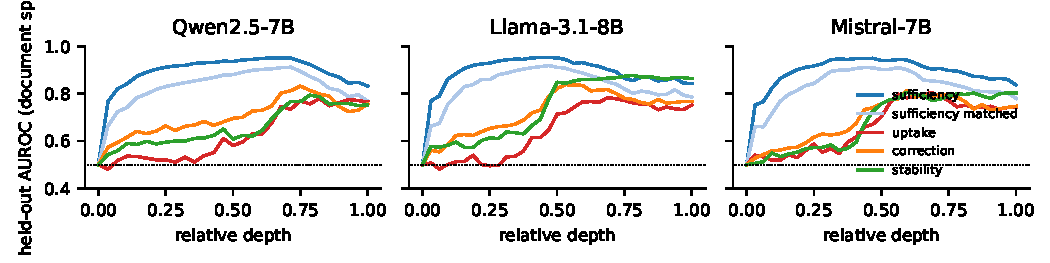
\includegraphics[width=0.84\linewidth]{auroc_by_layer}
\caption{Held-out AUROC by relative depth for the update tasks (document split). Sufficiency peaks around mid-depth in every model; uptake and correction emerge later.}
\label{fig:layers}
\end{figure*}

\paragraph{Sufficiency is linearly readable and robust.}
A probe trained to recognise the decisive increment, the one that adds the last missing paragraph, separates it from all other increments at $0.948$--$0.952$ AUROC in the three models (\cref{tab:probes}). The signal is strongest at 50--60\% of the network's depth (\cref{fig:layers}). The harder test compares the decisive increment only with its four \emph{matched controls}, which start from the same context with one paragraph missing and add, instead of that paragraph, a length-matched distractor, a duplicate of a paragraph already present, a falsified copy of the missing paragraph, or an irrelevant paragraph that mentions the answer string. Against these controls the probe still reaches $0.91$--$0.92$. Surface properties do not explain the result either. A classifier that sees only the nuisance covariates reaches $0.86$--$0.87$, adding the probe score to it gains $0.11$--$0.12$, and a probe trained after the covariates have been regressed out of the activations still reaches $0.94$--$0.96$. The result does not depend on how questions are split between training and test: splits that keep questions, supporting documents, answer entities or relation types disjoint all give $0.94$--$0.96$ (\cref{tab:splits}). The state-sufficiency probe, which classifies whole contexts rather than transitions, reaches $0.99$, but part of that comes from paragraph count; \cref{sec:what} separates the two.

\Cref{fig:kinds} projects held-out increments onto the sufficiency direction, that is, it computes their score along the probe's weight vector. The kinds of increment are ordered as one would expect if the direction encoded ``the evidence has just become complete'': decisive $>$ false $>$ distractor $>$ duplicate $>$ answer-string control $>$ a gold paragraph that does not yet complete the evidence. Increments added after the context is already sufficient, and the first hop, score far below. The falsified paragraph scoring second indicates that the direction encodes ``the final slot has been filled'' rather than truth, which is all the model can register before it generates.

\begin{figure}[t]
\centering
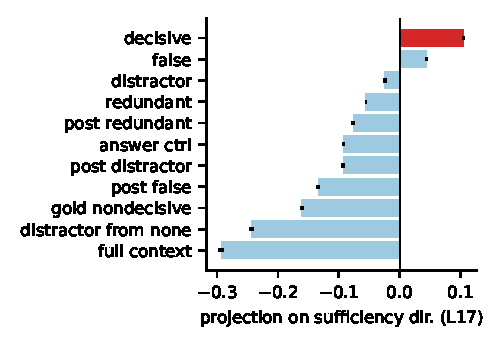
\includegraphics[width=\linewidth]{projection_by_kind}
\caption{Mean projection of held-out increments on the sufficiency direction, by kind of increment (Qwen2.5-7B, document split; standard errors). Red: decisive.}
\label{fig:kinds}
\end{figure}

\paragraph{Uptake is a separate, later signal.}
Among decisive increments, a probe can also predict whether the model will use the new paragraph, that is, whether its answer becomes correct, or will ignore it. This uptake probe reaches $0.77$--$0.78$ AUROC on the document split and $0.85$ on the question split, at layers near the end of the network. Uptake is also the task where the activations add most beyond surface properties ($+0.14$ to $+0.21$ over the nuisance classifier). It is a different signal from sufficiency. The two directions are nearly orthogonal (cosine $0.02$--$0.03$), and the sufficiency direction scores only $0.54$--$0.60$ when used to predict uptake. Uptake does share a direction with \emph{correction}, the transition from a wrong or abstaining answer to a correct one (cosine $0.30$--$0.34$; each direction predicts the other task at $0.82$ AUROC; \cref{fig:transfer}, \cref{app:transfer}). Correction and stability, by contrast, are largely predictable from the change in the model's output distribution. Nuisance-only classifiers, which include that change, reach $0.81$--$0.85$ on correction and $0.90$--$0.92$ on stability, and the probe adds at most $0.06$.

\paragraph{Transfer.}
We also apply the directions learned on 2-hop \musique{} questions, without retraining, to three other settings (\cref{tab:transfer}, \cref{app:transfer}). The first is the conversational protocol, in which the model sees its previous answer before the new paragraph. There the directions reach $0.79$ (sufficiency), $0.78$ (uptake), $0.92$ (correction) and $0.82$ (stability). This supports the view that the transition is intrinsic to evidence integration, rather than an artefact of the stateless design, in which each context is processed afresh, or of being asked to reconsider an answer. The second is \twowiki{}, where the sufficiency direction reaches $0.96$ ($0.93$ against matched controls), correction $0.85$ and uptake $0.79$, against $0.99$, $0.89$ and $0.91$ for probes trained on \twowiki{} itself. The third is 3--4-hop \musique{} questions, where sufficiency transfers at $0.82$--$0.85$. Probes trained on the 3--4-hop questions reach $0.93$ for sufficiency on every split and score the completion of a leave-one-out context as high as the completion of a chain (\cref{app:multihop}). Their uptake readout is less robust: it falls to $0.61$ on the document and answer splits, from $0.80$ on the question and relation splits.

\subsection{What the probes read: state, update and output}
\label{sec:what}
Two alternative explanations could account for a high sufficiency AUROC on paired updates. The first is that the update itself is incidental: the information may already be present in the absolute state after (or before) the new evidence, and subtracting the two states would then add nothing. The second is that the probe is simply reading the model's planned output. The anchor is the position from which the first answer token is predicted, and the prompt offers INSUFFICIENT as the alternative to answering. A sufficiency probe could therefore be reading ``about to say INSUFFICIENT'' rather than any comparison between the evidence and the question. We test both explanations on the same increments, labels and splits.

\paragraph{State versus update.}
We refit every update probe on four representations of the same increments: the state before the new evidence $h(C_{k-1})$, the state after it $h(C_k)$, their difference $\Delta h$, and their concatenation $[h(C_{k-1});h(C_k)]$ (\cref{tab:rep_ablation}, \cref{app:rep}). Most of the sufficiency readout is a property of the state \emph{after} the new evidence. $h(C_k)$ alone reaches $0.930$--$0.940$, against $0.947$--$0.952$ for $\Delta h$ (matched controls: $0.900$--$0.908$ against $0.910$--$0.917$). The state before the evidence reaches $0.733$ in all three models. This is exactly the AUROC of an oracle that knows only the stage at which the increment starts, namely empty, partial or already sufficient: decisive increments make up $20\%$ of the increments that start from a partial context and none of the others. So $h(C_{k-1})$ contributes nothing beyond that stage, and on the matched task, where the decisive increment and its four controls share their starting context, it scores exactly $0.500$. The concatenation matches $\Delta h$ ($0.949$--$0.950$). The subtraction therefore adds no information beyond having both endpoints. What it does is remove the question-specific content that both states share, so that a single linear direction works across questions.

For uptake, correction, stability and revision, the state after the evidence is as good as the update or better (uptake $0.769$--$0.798$ against $0.771$--$0.783$; stability $0.813$--$0.882$ against $0.750$--$0.869$). One caveat applies to $h(C_k)$ on the sufficiency task. A detector of ``is this context sufficient?'' is not enough, because $27\%$ of the negative increments add evidence to a context that is already sufficient. Indeed, the state-sufficiency probe applied to $h(C_k)$ of the same increments scores only $0.70$. The update probes solve a different task: ``has the context \emph{just} become sufficient?''. In short, the model's state represents whether its context has just become sufficient, and the paired update is a clean way to read that. The paired design is what makes the comparison controlled, through matched controls that share a starting context and through the causal tests of \cref{sec:causal}. It is not what makes the information readable.

\paragraph{Evidence versus output.}
The model's output is itself a sufficiency judgement: it answers when it judges the evidence sufficient and says INSUFFICIENT otherwise. That judgement is often wrong on sufficient evidence. On held-out contexts that contain every gold paragraph, the model says INSUFFICIENT $33\%$ (Qwen), $40\%$ (Llama) and $43\%$ (Mistral) of the time (\cref{tab:behaviour}). Read as a sufficiency classifier, the output reaches only $0.68$--$0.76$ AUROC. The state-sufficiency probe, read at the anchor of the same forward pass, reaches $0.99$. That figure is inflated, because every context with three or more paragraphs is sufficient. We therefore retrain the probe on two-paragraph contexts only, comparing minimal sufficient contexts with every other two-paragraph context, so that paragraph count cannot help. It still reaches $0.976$--$0.986$, against $0.71$--$0.77$ for the model's own answers (\cref{tab:verbal_internal}, \cref{app:behaviour}).

The probe is also accurate where the model's judgement fails. Restricted to the contexts on which the model says INSUFFICIENT, it still separates sufficient from insufficient ones at $0.967$--$0.982$. With its threshold set for $0.95$ precision on training data, it recovers $76$--$81\%$ of the sufficient contexts the model wrongly rejected, with $3$--$4\%$ false alarms on the insufficient contexts the model correctly rejected. The sufficiency update probes behave the same way when the output is held fixed: trained and tested only on increments after which the model \emph{still} says INSUFFICIENT, they reach $0.935$--$0.944$, against $0.65$--$0.69$ for the output alone (\cref{tab:behaviour_control}). The sufficiency readout is therefore not the planned output. The residual stream registers that the evidence has become complete even in cases where the model's own answer denies it.

The internal signal is weaker in those cases, though. On a scale where the mean probe score of insufficient training contexts is $0$ and that of sufficient ones is $1$, wrongly rejected contexts score $0.80$--$0.87$, against $1.03$ for sufficient contexts the model answers. The internal state is graded, and the verbal decision behaves like a thresholded, noisier read-out of it. This gap between registering complete evidence and acting on it is what uptake measures. It also explains why better sufficiency detection does not by itself buy accuracy in adaptive retrieval (\cref{app:adaptive}): stopping retrieval at a sufficient context the model will not answer from still yields INSUFFICIENT.

\subsection{Is the internal state needed? Text-only baselines}
\label{sec:text}
An obvious objection is that a text classifier given the same inputs might do as well as the activation probe. \Cref{tab:text} trains three such classifiers on the same increments, labels and splits: a TF-IDF logistic regression and two fine-tuned DeBERTa-v3 classifiers \cite{he2023debertav3}, one that sees the question and the added paragraph and one that also sees the previous context. For sufficiency, TF-IDF reaches $0.62$ and the DeBERTa without context $0.72$--$0.73$. The DeBERTa with context reaches $0.89$--$0.92$ with a reduced training budget (one epoch, 256 tokens, 8k increments) and $0.97$ with the full budget (two epochs, 512 tokens, all increments), which exceeds the probe's $0.95$ on the same split. Sufficiency is therefore largely recoverable from the text: the activation probe is an accurate readout of a property the input already determines. Uptake is the opposite case. On the same increments no text classifier exceeds $0.63$ in predicting whether the model will use the decisive paragraph (Qwen $0.56$ with the reduced and $0.63$ with the full budget, Llama $0.52$, Mistral $0.60$, all with context), while the activation probes reach $0.77$--$0.78$. Whether evidence is taken up depends on the model's internal state, not on the evidence alone.

\begin{table*}[t]
\centering\small
\setlength{\tabcolsep}{4pt}
\begin{tabular}{lllcccc}
\toprule
Model & Budget & Task & TF-IDF & DeBERTa (q+added) & DeBERTa (+context) & Probe \\
\midrule
Qwen2.5-7B & reduced budget & sufficiency & 0.623 & 0.723 & 0.900 & 0.948 \\
Qwen2.5-7B & reduced budget & sufficiency matched & 0.623 & 0.758 & 0.823 & 0.911 \\
Qwen2.5-7B & reduced budget & uptake & 0.574 & 0.569 & 0.557 & 0.775 \\
Qwen2.5-7B & full budget & sufficiency & 0.611 & 0.723 & 0.972 & 0.948 \\
Qwen2.5-7B & full budget & uptake & 0.574 & 0.625 & 0.630 & 0.775 \\
Llama-3.1-8B & reduced budget & sufficiency & 0.625 & 0.715 & 0.888 & 0.952 \\
Llama-3.1-8B & reduced budget & uptake & 0.463 & 0.466 & 0.517 & 0.783 \\
Mistral-7B & reduced budget & sufficiency & 0.625 & 0.730 & 0.920 & 0.949 \\
Mistral-7B & reduced budget & uptake & 0.536 & 0.573 & 0.604 & 0.771 \\
\bottomrule
\end{tabular}
\caption{Text-only classifiers trained on the same increments and splits as the activation probe (document split). ``q+added'': the classifier sees the question and the added paragraph; ``+context'': it also sees the previous context.}
\label{tab:text}
\end{table*}
